\documentclass[a4paper,12pt]{article}
\usepackage[utf8]{inputenc}
\usepackage[T1]{fontenc}
\usepackage[francais]{babel}
\usepackage{graphicx}
\usepackage[left=3cm,right=3cm,top=4cm,bottom=4cm]{geometry}
\pagestyle{plain}

\title{Projet d'Optimisation Numérique : \\ \smallskip \Large Méthodes numériques pour les problèmes d'optimisation \\ \bigskip}
\author{Grégoire Martini 2ING}
\date{Mardi 9 Février 2016}

\begin{document}
\maketitle
\tableofcontents
\newpage

\section{Optimisation sans contraintes}

\subsection{Algorithme de Newton local}

L'algorithme implémenté converge en une seule itération pour la fonction de test f1 car le gradient de celle-ci est linéaire et donc sa hessienne est constante. Ainsi le calcul de la première direction de Newton amène directement au point de gradient nul qui est unique (f1 strictement convexe car sa hessienne est définie positive).\\

L'algorithme peut en revanche ne pas converger pour la fonction de test f2 car la hessienne de celle-ci peut ,en fonction du point où elle est évaluée, ne pas être définie positive. La méthode utilisée ici n'est alors pas bien définie et l'algorithme peut diverger.\\


\subsection{Régions de confiance}

Le modèle de Taylor de la fonction f1 à l'ordre 2 est égale à la fonction car celle-ci est une quadratique. Le pas de Cauchy est une méthode qui approche la fonction par un modèle quadratique qui est donc ici égale à la fonction. On peut donc comparer l'algorithme de Newton local à celui de la région de confiance avec le pas de Cauchy. \\

On remarque ainsi que la région de confiance avec le pas de Cauchy ne converge pas aussi souvent que Newton local (notamment pour f2) et nécessite dans tout les cas plus d'itérations pour arriver à la solution (notamment pour f1). 
Néanmoins, la région de confiance avec Moré-Sorensen permet de converger pour f2(x023) alors que les autres algorithmes ne le permettent pas. \\

L'avantage de More-Sorensen est d'être une méthode exacte alors que le pas de Cauchy est une méthode approchée qui utilise un modèle quadratique. L'inconvénient est la complexité de l'algorithme et donc du calcul alors que le pas de Cauchy est très simple.\\

\begin{center}
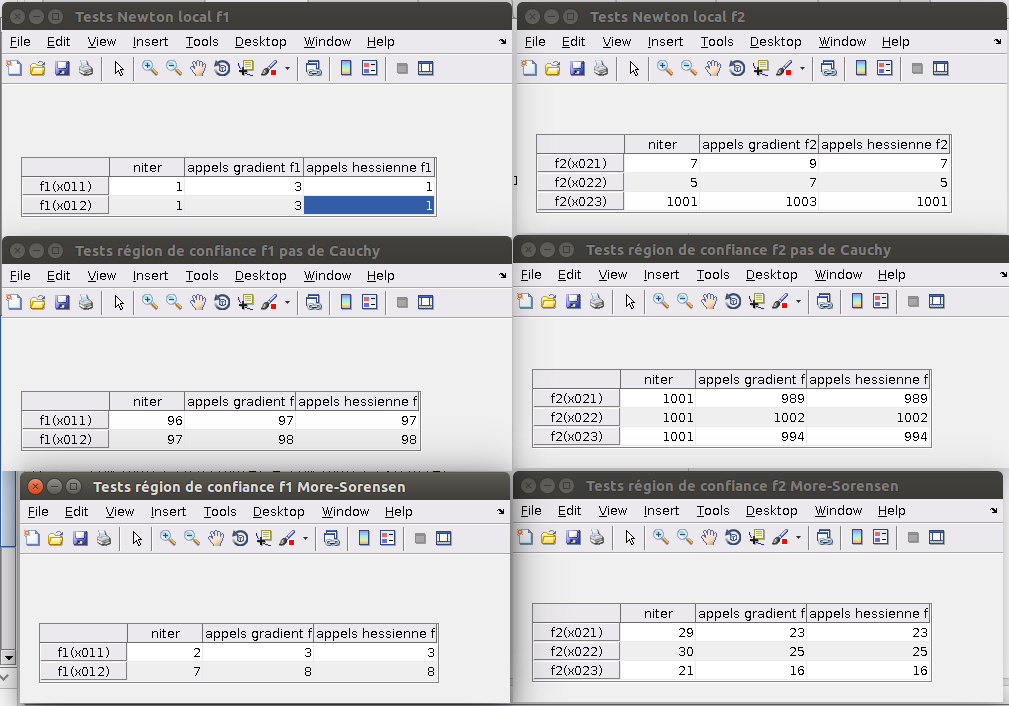
\includegraphics[width=14cm]{q3.png}
\end{center}

Pour modifier la vitesse de convergence de la région de confiance on peut modifier delta\_max la taille maximale de la région de confiance, gamma\_1 et gamma\_2 les facteurs de modification de la taille de la région de confiance et eta\_1 et eta\_2 les seuils de modification de la taille de la région de confiance. On obtiens entre autres les résultats suivant:\\

\begin{center}
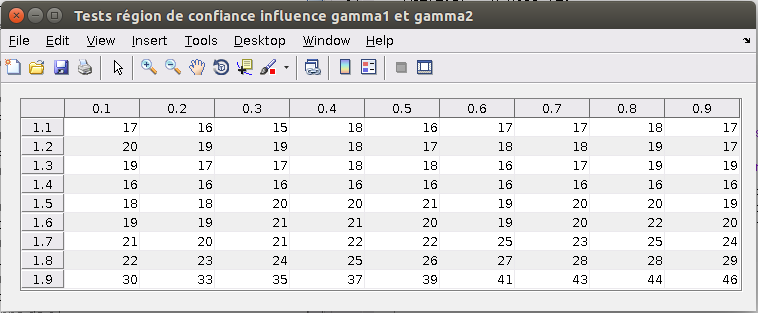
\includegraphics[width=14cm]{q4.png}
\end{center}

On observe ainsi que la diminution de gamma\_1 et gamma\_2 réduit globalement le nombre d'itérations de l'algorithme.

\clearpage
Le seul critère d'arrêt pertinent pour la méthode de Newton pour les équations non linéaires est la distance à la solution (f(x)=0). On peut utiliser la distance des bornes de la dichotomie à la solution comme bonne approximation si tenté que lambda\_min ou lambda\_max n'est pas égale à la solution au départ. Grâce à la dichotomie il ne peut y avoir de stagnation.\\

Dans le cas où l'utilisateur ne fournit pas de couple lambda\_min lambda\_max vérifiant la condition, on peut augmenter la zone lambda\_min lambda\_max en diminuant lambda\_min et augmentant lambda\_max jusqu'à vérifier la condition.\\


\section{Optimisation avec contraintes}

\subsection{Lagrangien augmenté}

Résultat

\begin{center}
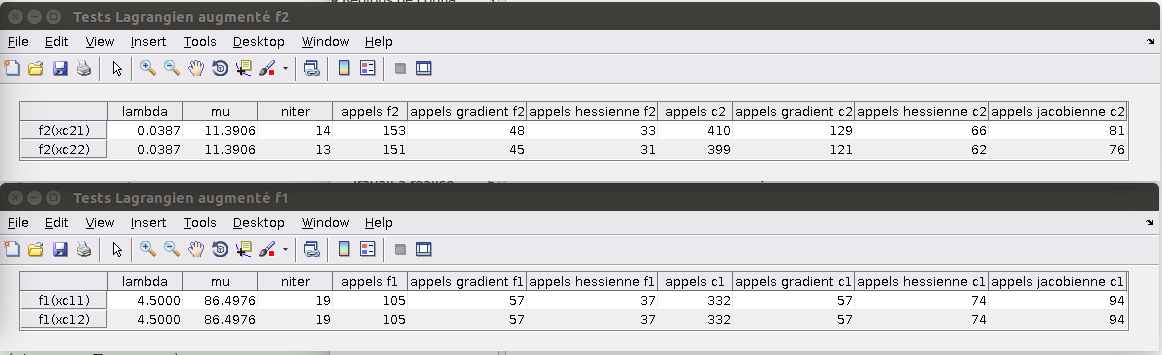
\includegraphics[width=14cm]{q5.png}
\end{center}

Influence de tau

\begin{center}
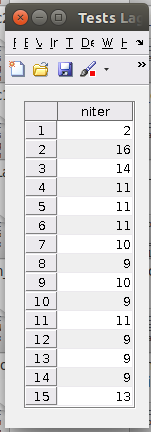
\includegraphics[height=8cm]{q6.png}
\end{center}

Au vu des résultats précédents, il semble difficile de déduire une influence précise de tau sur la performance de l'algorithme.\\

Supplément.
Sans modifier l'algorithme, on peut transformer les contraintes d'inégalité en contraintes d'égalité en ajouter une variable réelle à la fonction contrainte dont le signe dépendra du sens de l'inégalité. On trouve ainsi une solution possible, il faut vérifier que le signe des variables est bien celui attendu, dans le cas contraire la solution est fausse et il faut utiliser une autre méthode pour trouver une solution.\\


\bigskip
Les performances des algorithme ont été ici étudiées en termes de nombre d'itérations. On aurait pu les étudier en termes de temps de calcul mais il aurait fallu supprimer les effets de bords qui pénalisent l’exécution.

\end{document}          
